% Some commands used in this file

\chapter{Pre-Survey and Experiment Findings}
The following chapter will give an overview of the data obtained from the survey, which was conducted before running the experiment.
Later, an overview of the data obtained from the experiment is explained along with feedback received from the participants. This chapter puts forth
all that was learnt from the above mentioned.


\section{Overview of the Pre-Survey Data}
The survey has 199 participants. After filtering out spurious and half-filled entries 189 of them are used for the analysis.



\section{Pre-Survey Methodology and Findings}
All the results presented below were performed on the data by performing the following changes to the data:
\begin{enumerate}
\item Rows with empty fields were removed
\item Rows with spurious data was removed
\item Data was scaled or normalized when necessary
\end{enumerate}

Other than the above, the data was not manipulated. Outliers were not excluded either.

\subsubsection{Perception of Individual Sensor Grouped on the Intrusion of Sensors in General}
We try to examine here if the perception of intrusion  of Sensors can affect the way a person views the individual sensors themselves. In other
words, we try to examine if there is a significant difference in perception of each sensor depending on the perception of the Sensors as a whole.
For this, we grouped the survey data based on the responses to question 10. Since there are 5 possible responses to this question, this makes 5 individual groups from 1 to 5.

We now have 5 groups who view sensors in a different light each and their perception of each of the individual sensors can be compared. Before going into the comparison, we try to understand the properties of the data. To perform a one-way ANOVA test or a t-test, the data needs to be:

\begin{enumerate}
\item Normally distributed
\item Homoscedastic
\item Ordinal or continuous
\end{enumerate}

Since the data is discrete and follows the Likert Scale with options from 1 to 5, it gives skewed normal distribution. Additionally, the variances of values within the groups formed are not similar. One-way ANOVA test is quite robust to heteroscedacity, as long as the maximum variance among all groups is less than four times the group with the lowest variance. The scale used to collect data is in the ordinal form. Accounting for all the violations, we instead opt for a non-parametric tests such as the Kruskal-Wallis H test and the Dunn's test
which only assume the following : 

\begin{enumerate}
\item Groups are independant from one another
\item All observations are independant
\item The dependant variables should be in the ordinal scale or continuous
\end{enumerate}

The above tests do not make any assumptions about the distribution of the data and are robust to heteroscedastic data.
\begin{figure}[htp]
\subtop[Mean of each Group for each Sensor\label{fig:s1}]{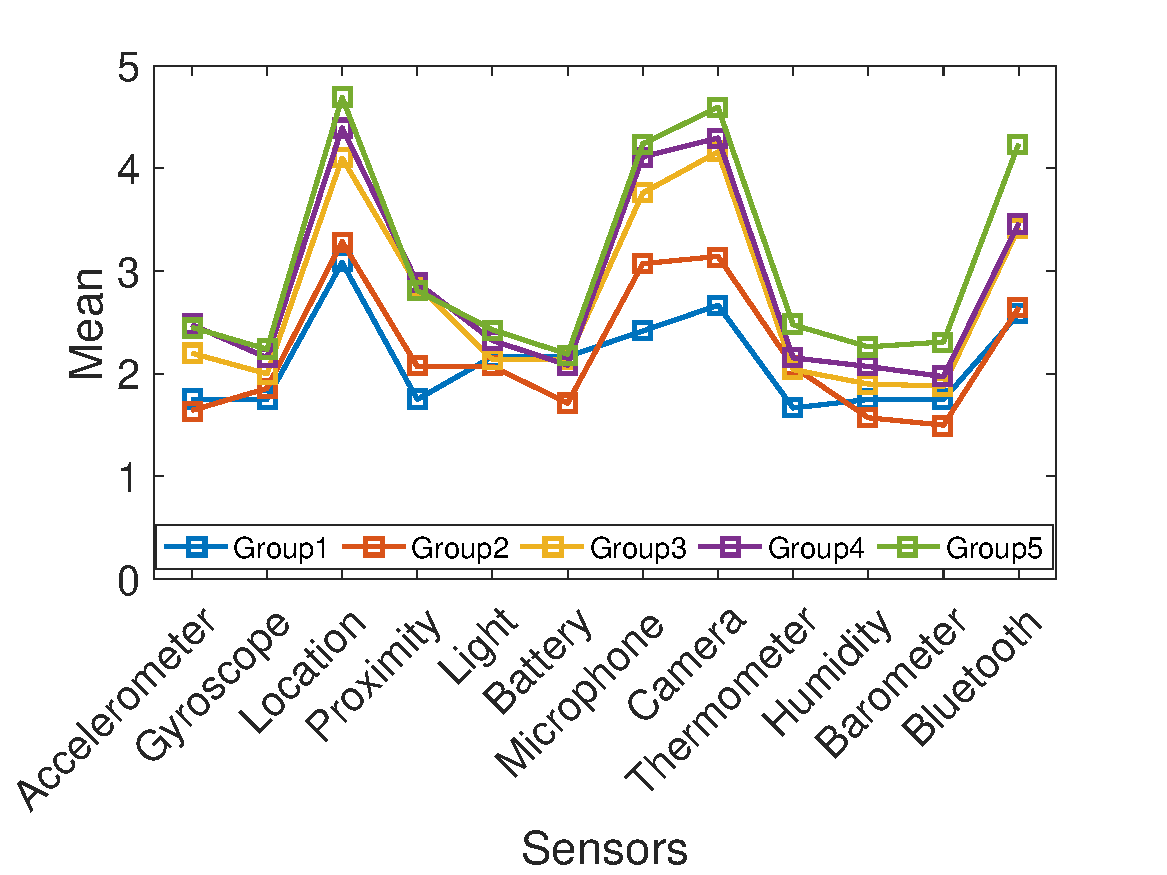
\includegraphics[width=0.55\linewidth]{./images/sensors_group_meanQ10}}
\subtop[Variance of each Group for each Sensor\label{fig:s2}]{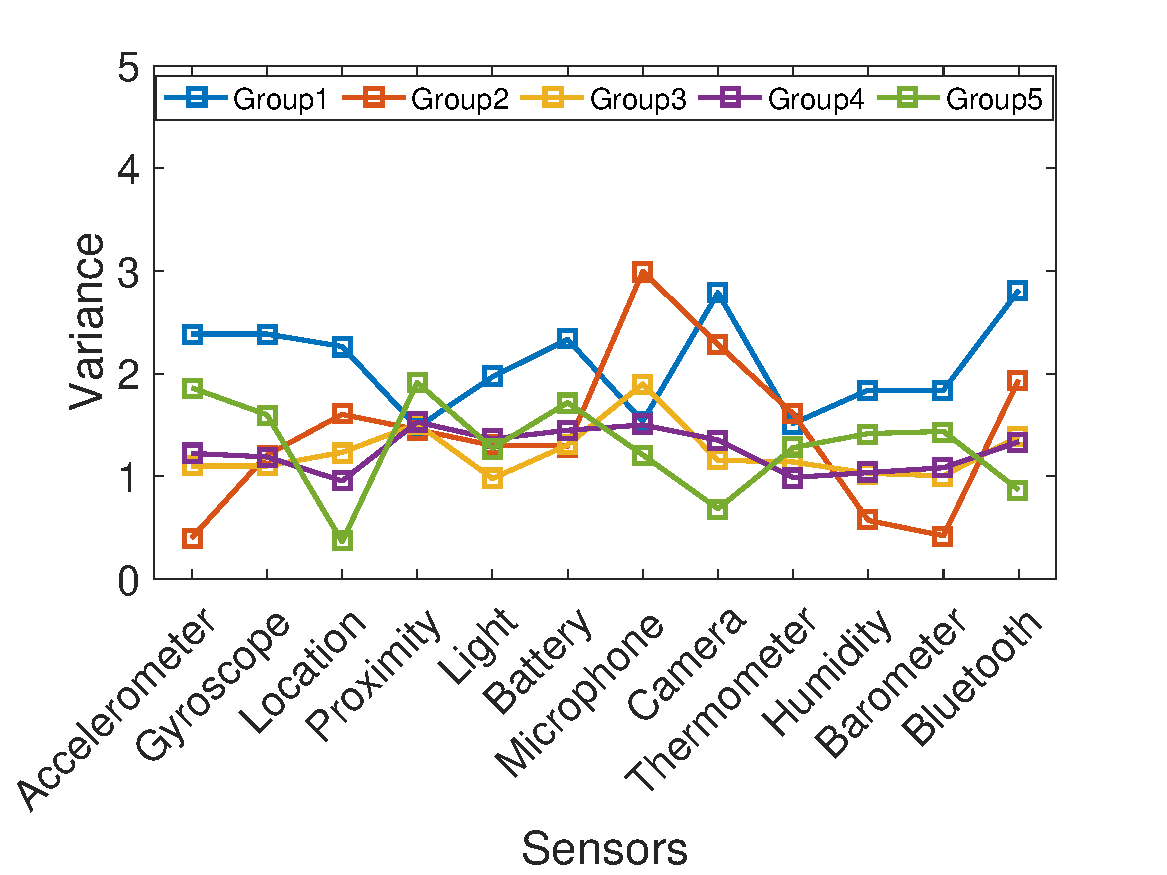
\includegraphics[width=0.55\linewidth]{./images/sensors_group_varianceQ10}}
\caption{Table Schemas}
\label{fig:s3}
\end{figure}

Group 1 to 5 have 13, 14, 50, 71 and 42 people each respectively. For in depth analysis of the composition of each group in terms of employment, education, gender and birth year please refer to tables
\ref{tab:emp_sensors},\ref{tab:edu_sensors},\ref{tab:gender_sensors},\ref{tab:year_sensors}. Figures \ref{fig:s1} and \ref{fig:s2} depict the mean and variances for each of the individual groups. We start by performing the non paramteric Kruskal-Wallis test on each Sensor. The value of alpha assumed here is 0.05. The null hypothesis states that all the groups perceive the sensors in the similar way. This means they come from the same distribution. The alternative hypothesis is
that the groups perceive each sensor in a significantly different way. The table \ref{tab:kw_sensors} depicts the p-values obtained from the test.


\begin{table}[h!]
  \centering
  \caption{Employment Classification of Groups}
  \label{tab:emp_sensors}
  \begin{tabular}{cccccc}
    \toprule
     Occupation&1&2&3&4&5\\
    \midrule
Employed full time&4.90\%&6.86\%&26.47\%&38.24\%&23.53\%\\
Employed part time&8.33\%&16.67\%&33.33\%&16.67\%&25.00\%\\
Unemployed and looking for work&8.33\%&16.67\%&16.67\%&25.00\%&33.33\%\\
Unemployed and not looking for work&0.00\%&0.00\%&0.00\%&66.67\%&33.33\%\\
Retired&0.00\%&0.00\%&100.00\%&0.00\%&0.00\%\\
Student&7.23\%&4.82\%&26.51\%&39.76\%&21.69\%\\
Disabled&0.00\%&0.00\%&0.00\%&0.00\%&0.00\%\\
    \bottomrule
  \end{tabular}
\end{table}



\begin{table}[h!]
  \centering
  \caption{Gender Classification of Groups}
  \label{tab:gender_sensors}
  \begin{tabular}{cccccc}
    \toprule
     Gender&1&2&3&4&5 \\
    \midrule
Female&5.56\%&4.17\%&33.33\%&30.56\%&26.39\% \\
Male&7.14\%&9.52\%&22.22\%&39.68\%&21.43\% \\
    \bottomrule
  \end{tabular}
\end{table}



\begin{table}[h!]
  \centering
  \caption{Average Birth Year of Groups}
  \label{tab:year_sensors}
  \begin{tabular}{ccccc}
    \toprule
     1&2&3&4&5\\
    \midrule
	1989& 1979& 1986& 1986& 1983\\
    \bottomrule
  \end{tabular}
\end{table}


\begin{table}[h!]
  \centering
  \caption{Education Classification of Groups}
  \label{tab:edu_sensors}
  \begin{tabular}{cccccc}
    \toprule
     Education&1&2&3&4&5\\
    \midrule
    
Less than high school&20.00\%&20.00\%&20.00\%&40.00\%&0.00\%\\
High school&10.53\%&0.00\%&52.63\%&31.58\%&5.26\%\\
Some college&10.00\%&20.00\%&30.00\%&20.00\%&20.00\%\\
Bachelors degree&7.02\%&10.53\%&24.56\%&42.11\%&15.79\%\\
Masters degree&3.80\%&5.06\%&24.05\%&35.44\%&31.65\%\\
PhD degree&7.14\%&7.14\%&17.86\%&35.71\%&32.14\%\\
    \bottomrule
  \end{tabular}
\end{table}  




\begin{table}[h!]
  \centering
  \caption{Kuskal-Wallis Test}
  \label{tab:kw_sensors}
  \begin{tabular}{cccc}
    \toprule
     Sensor & p-value \\
    \midrule
    Accelerometer & 0.0151 \\
    Gyroscope & 0.2959\\
    Location & 1.0664e-05\\
    Proximity & 0.0147\\ 
    Light & 0.6933\\
    Battery & 0.6950\\ 
    Microphone & 3.0070e-04\\
    Camera & 2.1191e-05\\
    Thermometer & 0.0693\\ 
    Air Humidity & 0.1292\\
    Barometer & 0.0949\\
    Bluetooth & 3.4877e-05\\ 
    \bottomrule
  \end{tabular}
\end{table} 

On these sensors, we proceed with a post hoc test by performing a pariwise Dunn's test to examine if there is an actual significant difference between the groups and if so between which groups. The sensors with p values with less than 0.05 are examined in more detail and the p-values are presented in table \ref{tab:dunn_sensors}. The table shows the results for each pairwise test done, with the p-values adjusted using the Bonferroni Method. The reason for choosing to adjust the p-values is that repeated experiments can increase the chances of accepting the alternative hypothesis so p-values are adjusted according to the number of experiments performed. 10 experiments are performed per sensor.

\begin{table}[h!]
  \centering
  \caption{Dunn's Test 1}
  \label{tab:dunn_sensors}
  \begin{tabular}{ccccccc}
    \toprule
     Groups & Accelerometer & Location & Proximity & Microphone & Camera & Bluetooh \\
    \midrule
    (1,2) & 1.0000 & 1.0000 & 0.9992 & 0.8365 & 1.0000 & 1.0000 \\
    (1,3) & 0.4207 & 0.2084 & 0.0699 & 0.0365 & 0.0732 & 0.7825 \\
    (1,4) & 0.0595 & 0.0125 & 0.0513 & 0.0012 & 0.0048 & 0.6442 \\
    (1,5) & 0.2054 & 0.0010 & 0.1191 & 0.0009 & 0.0007 & 0.0029 \\
    (2,3) & 0.6548 & 0.1774 & 0.3713 & 0.8927 & 0.1694 & 0.5921 \\
    (2,4) & 0.1185 & 0.0077 & 0.2617 & 0.2287 & 0.0123 & 0.4270 \\
    (2,5) & 0.3659 & 0.0005 & 0.5184 & 0.1597 & 0.0018 & 0.0007 \\
    (3,4) & 0.8989 & 0.7642 & 1.0000 & 0.8052 & 0.9040 & 1.0000 \\
    (3,5) & 0.9997 & 0.0869 & 1.0000 & 0.6390 & 0.2947 & 0.0066 \\
    (4,5) & 0.9998 & 0.8360 & 1.0000 & 1.0000 & 0.9617 & 0.0059 \\
    \bottomrule
  \end{tabular}
\end{table} 

For the Accelerometer and Proximity, we can see that none of the pairwise groups have a significant difference from each other. This means that even tough the groups perceive sensors differently in general, they all view Accelerometers and Proximity in a similar way. 

For the location sensor, it can be observed that groups (1,4), (1,5), (2,4), (2,5) have a significant difference. This can be attributed to the fact that since the groups are formed from the perception of people of the Sensors Feature, the difference in perception between group 1 and group 5 will be larger than between group 1, group 2 and group 1, group3 since they are not much apart in the scale.

For the microphone sensor, it can be seen that groups (1,3), (1,4) and (1,5) are significantly different from each other. This goes to show that
if people rate sensors as even a little intrusive, they all rate the microphone's in a significantly different way than the people who rate sensors as non-intrusive.

For the camera sensor, it can be observed that groups (1,4), (1,5), (2,4), (2,5) have a significant difference in their perception of the intrusion.
Similar to the location sensor, people with perception of sensors in general with a lower intrusion level have significantly different responses to the camera intrusion than the people who rate sensors with more intrusion.

For the Bluetooth sensor, there is a significant difference between groups (1,5), (2,5), (3,5) and (4,5). This shows that responses by people who find sensors extremely intrusive is different from the rest of the groups.

\subsubsection{Perception of Individual Stakeholders Grouped on the Intrusion of Stakeholders in General}

In this section, we try to see if the intrusion level perception by people of Stakeholders in general and the intrusion of the individual stakeholders are related. We try to examine significant differences between groups formed by using question 12 responses of the survey ranging from one to five for every Stakeholder. 

\begin{table}[h!]
  \centering
  \caption{Employment Classification of Groups}
  \label{tab:emp_stak}
  \begin{tabular}{cccccc}
    \toprule
     Occupation&1&2&3&4&5\\
    \midrule
Employed full time	&3.92\%	&4.90\%	&16.67\%	&33.33\%	&41.18\%\\
Employed part time	&16.67\%	&16.67\%	&8.33\%	&50.00\%	&8.33\%\\
Unemployed, looking for work	&8.33\%	&8.33\%	&16.67\%	&16.67\%	&50.00\%\\
Unemployed, not looking for work	&0.00\%	&0.00\%	&0.00\%	&33.33\%	&66.67\%\\
Retired	&0.00\%	&0.00\%	&0.00\%	&100.00\%&	0.00\%\\
Student	&4.82\%	&7.23\%	&15.66\%	&37.35\%	&34.94\%\\
Disabled	&0.00\%	&0.00\%	&0.00\%	&0.00\%	&0.00\%\\
    \bottomrule
  \end{tabular}
\end{table}



\begin{table}[h!]
  \centering
  \caption{Gender Classification of Groups}
  \label{tab:gender_stak}
  \begin{tabular}{cccccc}
    \toprule
     Gender&1&2&3&4&5 \\
     \midrule
Female&5.56\%&6.94\%&23.61\%&36.11\%&27.78\% \\
Male&3.97\%&6.35\%&11.90\%&35.71\%&42.06\%\\
    \bottomrule
  \end{tabular}
\end{table}



\begin{table}[h!]
  \centering
  \caption{Average Birth Year of Groups}
  \label{tab:year_stak}
  \begin{tabular}{ccccc}
    \toprule
     1&2&3&4&5\\
    \midrule
	1986& 1989& 1984& 1985& 1984\\
    \bottomrule
  \end{tabular}
\end{table}


\begin{table}[h!]
  \centering
  \caption{Education Classification of Groups}
  \label{tab:edu_stak}
  \begin{tabular}{cccccc}
    \toprule
     Education&1&2&3&4&5\\
    \midrule
    
Less than high school	&20.00\%	&20.00\%	&0.00\%	&60.00\%	&0.00\%\\
High school	& 15.79\%&	5.26\%	&21.05\%	&31.58\%	&26.32\%\\
Some college	 & 0.00\%&	10.00\%	&20.00\%	&40.00\%&	30.00\%\\
Bachelors degree 	&1.75\%	&12.28\%&	15.79\%	&35.09\%	&35.09\%\\
Masters degree	&5.06\%	&1.27\%	&13.92\%	&37.97\%	&41.77\%\\
PhD degree	&0.00\%	&7.14\%	&21.43\%	&28.57\%	&42.86\%\\
    \bottomrule
  \end{tabular}
\end{table} 



\subsubsection{Perception of Individual Contexts Grouped on the Intrusion of Contexts in General}

\section{Overview of the Experiment Data}

\section{Findings from the Experiment Data}



